\documentclass{extarticle}
\usepackage[a4paper,left=1in,right=1in,bottom=1in]{geometry}
\usepackage[parfill]{parskip}
\usepackage{ragged2e}
\usepackage{amsmath} 
\usepackage{amsthm} 
\usepackage{graphics}
\usepackage{amssymb}
\usepackage{upgreek}
\usepackage{listings}
\usepackage{esint}
\usepackage{floatrow}
\newtheorem{theorem}{Theorem}
\newtheorem{lemma}{Lemma}
\newtheorem{corollary} [theorem] {Corollary}
\newtheorem{proposition}{Proposition}[section]
\theoremstyle{remark}
\newtheorem*{remark}{Remark}
\usepackage[ruled,linesnumbered,vlined]{algorithm2e}
\usepackage{xcolor}
\usepackage{listings}
\usepackage{color}
\definecolor{name}{rgb}{0.5,0.5,0.5}
\usepackage{hyperref}
\usepackage{url}
\usepackage{multirow}
\usepackage{fancyhdr}
\usepackage{graphicx}
\newcommand{\y}[1]{\mathcal{O}(#1)}
\pagestyle{fancy}
\usepackage{pgfplots} 
\pgfplotsset{compat=newest} 

\fancyhf{}
%\setlength{\parindent}{7em} 
\lhead{190050043-190050055-190050077-190050079}
\rhead{Assignment-1}
\cfoot{Page \thepage}
\renewcommand{\footrulewidth}{1pt}
\newcommand{\tbf}[1]{\textbf{#1}}
\setcounter{tocdepth}{2}
\usepackage[utf8]{inputenc}
\begin{document}
\title{Assignment-1}
\author{190050043,190050055,190050077,1900500079}
\date{January, 2021}
\maketitle
%\tableofcontents
\thispagestyle{empty}
\clearpage
\pagenumbering{arabic}

\sffamily
\Large{Question 1}\\

\normalsize
a) Choosing the course x that ends last, discard classes that conflict with x,
and recurse.
\newline
\newline
\begin{center}

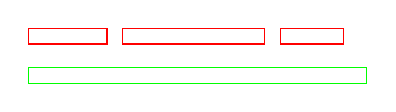
\begin{tikzpicture} 

\color{red}
\draw (1,0) rectangle (2,0.2);\draw (2.2,0) rectangle (4,0.2);
\draw (4.2,0) rectangle (5,0.2);
\color{green} \draw (1,-0.5) rectangle (5.3,-0.3);
\end{tikzpicture}
    
\end{center}
\vspace{0.2in}

for the above case our algorithm will select only one course (green since it ends late) . but optimal schedule is 3 courses ( courses in red)
\\



b) Choosing the course x that starts first, discard classes that conflict with x,
and recurse.
\newline
\newline
\begin{center}

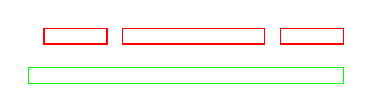
\begin{tikzpicture} 

\color{red}
\draw (1.2,0) rectangle (2,0.2);\draw (2.2,0) rectangle (4,0.2);
\draw (4.2,0) rectangle (5,0.2);
\color{green} \draw (1,-0.5) rectangle (5,-0.3);
\end{tikzpicture}
    
\end{center}
\vspace{0.2in}
for the above case our algorithm will select only one course (green since it starts first) . but optimal schedule is 3 courses ( courses in red)
\\

d) Choosing the course x with shortest duration, discard all classes that
conflict with x, and recurse.
\newline
\newline
\begin{center}

\begin{tikzpicture} 

\color{green} \draw (3.2,0) rectangle (5,0.2);
\color{red} \draw (2.7,-0.4) rectangle (3.4,-0.2);
\color{green} \draw (1,-0.9) rectangle (2.9,-0.7);
\end{tikzpicture}
    
\end{center}
\vspace{0.2in}
for the above case our algorithm will select only one course (red since it is shortest duration). but optimal schedule is 2 courses ( courses in green)\\

e) Choose a course x that conflicts with the fewest other courses, discard all classes that conflict with x, and recurse.\newline
\newline
\begin{center}

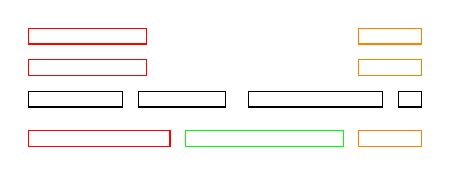
\begin{tikzpicture} 
\color{red}
\draw (1,0.4) rectangle (2.5,0.6);\draw (1,0.8) rectangle (2.5,1);
\color{black} \draw (1,0) rectangle (2.2,0.2);\draw (2.4,0) rectangle (3.5,0.2);\draw (3.8,0) rectangle (5.5,0.2);\color{green} \draw (3,-0.5) rectangle (5,-0.3);\color{red} \draw (1,-0.5) rectangle (2.8,-0.3); \color{orange} \draw (5.2,0.4) rectangle (6,0.6);\draw (5.2,0.8) rectangle (6,1);\draw (5.2,-0.5) rectangle (6,-0.3);;\color{black}  \draw (5.7,0) rectangle (6,0.2);
\end{tikzpicture}
\end{center}
\vspace{0.2in}

For the above case our algorithm choose only 3 courses. our algorithm selects course in green as green course conflicts with only 2 and in next recursion we select one course from red and discards rest and in next to next step selects one from orange and discards rest.
\newline
But the optimal is 4 courses ( all Black courses).

f) If no classes conflict, choose them all. Otherwise, discard the course
with longest duration and recurse.
\newline
\newline
\begin{center}

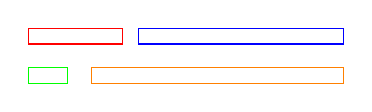
\begin{tikzpicture} 

\color{red}
\draw (1,0) rectangle (2.2,0.2);\color{blue} \draw (2.4,0) rectangle (5,0.2);

\color{green} \draw (1,-0.5) rectangle (1.5,-0.3);\color{orange} \draw (1.8,-0.5) rectangle (5,-0.3);
\end{tikzpicture}
    
\end{center}

for the above case our algorithm will select only one course (green ).First it will discard longest course(orange).As there is still a conflict it removes longest course(blue). Again it discards longest course (RED) hence only 1 course left and it is selected .but optimal schedule is 2 courses ( courses in green and blue )\\

g) If no classes conflict, choose them all. Otherwise, discard a course that
conflicts with the most other courses and recurse.
\newline
\newline
\begin{center}

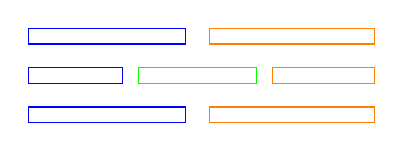
\begin{tikzpicture} 

\color{blue}
\draw (1,0) rectangle (2.2,0.2);\color{green} \draw (2.4,0) rectangle (3.9,0.2); \color{orange}\draw (4.1,0) rectangle (5.4,0.2);
\color{blue}
\color{orange} \draw (3.3,-0.5) rectangle (5.4,-0.3);\draw (3.3,0.5) rectangle (5.4,0.7);
\color{blue} \draw (1,-0.5) rectangle (3,-0.3);\draw (1,0.5) rectangle (3,0.7);
\end{tikzpicture}
\end{center}
\vspace{0.2in}
For the above case our algorithm chooses only 2 courses.At first it discards course which has conflict with most courses (Green).Then still there is conflict it removes either blue or orange and then finally selects one from blue and one from orange there will be 2 courses without conflicts hence chosen.
  But optimal solution takes 3 courses ( blue, Green , Orange in middle row).\\
  
c) Choose the course x that starts last, discard all classes that conflict
with x, and recurse.\\

\textbf{Correctness of the  heuristic:}\\

Let $ i_k, i_{k-1}, . . . , i_1 $ be the jobs selected by A.\\
Let $ j_m, j_{m-1}, . . . , j_1 $ be the jobs selected by OPT.\\
Lemma
For all r $\leq$ k, f ($i_r$ ) $\geq$ f ($j_r$).   ( Where f(x) is start time of job x )\\

Let us prove by induction\\
For r = 1, by the choice of $i_1$, f ($i_1$) $\geq$f ($j_1$).\\ 
Suppose $f (i_{r-1}) \geq f (j_{r-1})$.\\

When A picks its k-r th course, jr 
is also available for our algorithm to choose from.Because start time of k-r+1 is greater than k-m+1 the course so if jr is picked by opt then it is indeed able to picked by over algorithm \\
Our algorithm picks course having max start time if start time of $j_r$ is maximum then it picks it.\\
hence $f (i_{r}) \geq f (j_{r})$

hence start time of $ i_m \geq j_m $
hence k $\geq$ m.
This also shows that the algorithm  gives an optimal solution.\\

\vspace{0.4 in}


h) Let x be the class with the earliest start time, and let y be the class with
the second earliest start time.\\
 Case 1 • If x and y are disjoint, choose x and recurse on everything but x.\\
 Case 2 • If x completely contains y, discard x and recurse.\\
 Case 3 • Otherwise, discard y and recurse.\\

\textbf{Correctness of the  heuristic:}\\

Let $ i_1, i_{2}, . . . , i_k $ be the jobs selected by A.\\
Let $ j_2, j_{2}, . . . , j_m $ be the jobs selected by OPT.\\
Lemma\\
For all r $\leq$ k, f ($i_r$ ) $\leq$ f ($j_r$).   ( Where f(x) is time taken to complete  xth job )\\

first let us prove our algorithm chooses only course that ends first in available list of courses. and discard courses clash with it.
Let us prove by induction\\
For r = 1,\\ 
Case 1 : As y having 2nd min start time and x,y are disjoint. hence x is the job         that completes 1st and clashes with no other course (since 2nd course starts after completion of 1st ) is chosen by our algorithm. so whatever algorithm chooses is course that ends first with no courses clashing with it.\\
            
            
case 2 : If x completely contains y we discard x.  y ends before x as y is contained in x.  so x is not the one which ends first since y ends first. And as it starts first even there is z which starts 1st x will clash with z as z is contained in x. So we discard only course clashes with course which ends first.


case 3 : As y  has starting time more than x and not contained in x so it must have end time greater than x. y is clearly not the course that ends first. even if there is course ends before end of x it has start time after y so it clashes with y.we discard y only courses clash with course that ends first.\\

For r = 1, by the choice of $i_1$, f ($i_1$) $\leq$f ($j_1$). ( Because our algorithm chooses course that ends first)\\ 

Suppose $f (i_{r-1}) \leq f (j_{r-1})$.\\

When A picks its r th course, jr 
is also available for our algorithm to choose from.Because start time of r-1 is greater than k-1 th course so if jr is picked by opt then it is indeed able to picked by over algorithm \\
Our algorithm picks course that ends first. if  $j_r$ is course ending first then it picks it.\\
hence $f (i_{r}) \leq f (j_{r})$\\

hence start time of $ i_m \leq j_m $\\
hence k $\geq$ m.\\
This also shows that the algorithm  gives an optimal solution.\\


i) If any course x completely contains another course, discard x and
recurse. Otherwise, choose the course y that ends last, discard all classes
that conflict with y, and recurse.
    
    we will prove that chosen course y not only ends last but also starts last.\\
    
Let us assume that there is course  z starts after y.As y ends last then the z should end before or equal to end time of y. then y is containing z but we have removed all courses containing other.At any intermediate point when we discard few courses which clashes with selected one then also same argument holds.\\

This is contradiction. Hence the course which  ends last is starts last.
Thus  the course by algorithm is like choosing course that ends last in original list of courses.\\

when we discard courses which conflicts with last starting course then it is same as discarding courses conflict with last ending course as we have already removed courses containing this course which also conflicts with last starting in original one.  

hence we have to prove that algorithm selecting course that starts last is optimal.Which is exactly part c of the problem. Hence proved. \\

This  shows that the algorithm gives an optimal solution
\newpage






















%%%%%%%%%%%%%%%%%%%%%%%%%%%%%%%%%%%%%%%%%%%%%%%%%%%%%%%%%%%%%%%%%%%%%%%%%%%%%%%%%%%%%%%%%%%%%%%%%%%%%%%%%%%%%%%%%%%%%%%%%%%%%%%%%%%%%%%%%%%%%%%%%%%%%%%%%
\newpage

% \begin{algorithm}[H]
%     \SetAlgoLined
%     \KwData{Graph,source}
%     \KwResult{Distances of each vertex from the source and starting edges of the shortest paths}
%     create priority queue Q of vertices of Graph //min-heap\\
%     \ForEach {vertex v in Graph}{
%     $dist[v] \gets \infty$\\
%     $prev[v] \gets \text{UNDEFINED}$\\
%     $\text{add} v \text{to} Q$ 
%     }
%     $dist[source] \gets 0$\\
%     \While{Q is not empty do}{
%     $u \gets Q.extract()$\\
%     \ForEach{neighbour v $\in$ Q of u}{
%     $alt \gets dist[u]+length(u,v)$\\
%     \If{alt $<$ dist[v]}{
%     $dist[v] \gets alt$\\
%     $prev[v] \gets u$
%     }
%     }
%     }
%     $\text{return} ~dist[],prev[]$
%     \caption{Dijkstra's Algorithm}
%     \end{algorithm}
%\LARGE{Question1}\\

\Large{Question 2}\\
\normalsize


Subset b) is the required optimal solution for the rest of the cases we can come up
with a counter example.\\
Consider question papers to be a tuple of \{$t_{i,1}$,$t_{i,2}$\} where $t_{i,1}$,$t_{i,2}$ mean the same as mentioned in the question.\\
\tbf{Counter Examples}:\\
For a):\\
Consider 2 question papers with the first paper \{10,3\} and the second paper be \{6,5\}.
Now According to this possible greedy strategy our answer would be 21 but we can see that 
the best possible answer would be 19.\\
For c) :\\
Consider 2 question papers with the first paper \{10,3\} and the second paper be \{6,5\}.
Now According to this possible greedy strategy our answer would be 21 but we can see that 
the best possible answer would be 19.\\
For d) : \\
Consider 2 question papers with the first paper \{10,5\} and the second paper be \{6,3\}.
Now According to this possible greedy strategy our answer would be 21 but we can see that 
the best possible answer would be 19.\\
For e) :\\
Consider 2 question papers with the first paper \{10,3\} and the second paper be \{6,5\}.
Now According to this possible greedy strategy our answer would be 21 but we can see that 
the best possible answer would be 19.\\

\tbf{Proof} : \\
We can see that since the computer does every task one by one order does not matter 
and the total time taken by the computer for correcting all the question papers is always 
the same i.e, $\sum_{i} t_{i,1}$.\\
So no matter what the order is of the question papers this remains same hence in order to 
minimize the total time taken we need to take question papers optimally in a way such that
the total time taken is minimum and such that the correction part done by the teachers must
be efficient.\\
So let us prove by contradiction of our algorithm.\\
Let us consider two question papers with paper-1 be \{$t_{i,1}$,a$\}$ and paper-2 be
\{$t_{j,1}$,b$\}$ and now for the sake of contradiction let us consider $b > a$.\\
Then let us calculate the time taken for the completion of correcting these two question papers
the time taken would be $t_{i,1} + t_{j,1} + max(max(0,a-t_{j,1}),b)$.\\

Here we know that $b > a$ so clearly $b > a - t_{j,1}$ since $t_{j,1} > 0$ therefore 
the total time taken will become $t_{i,1} + t_{j,1} + b$.\\

Now let us analyze what happens when we swap the two question papers such that the ordering changes
to \{$t_{j,1}$,b$\}$ and \{$t_{i,1}$,a$\}$ .Now let us calculate the total time taken in this 
case .\\
The time taken would be $t_{j,1} + t_{i,1} + max(max(0,b-t_{i,1}),a)$.\\
Now let us consider 3 cases :\\
Case i) When $a > b-t_{i,1}$ :\\
Then we can see that the total time taken $t_{j,1} + t_{i,1} + a$ is cleary greater than the previous case
without swapping because $b > a$.\\
Case ii) When $a < b-t_{1,1}$ : \\
Now the total time would become $t_{j,1} + t_{i,1} + b - t_{i,1}$ which is $t_{j,1} + b$ which is less than the previous case 
because $t_{i,1} > 0$.\\
Case iii) When $b-t_{i,1} < 0$ : \\
Now we can cleary see that $ a > 0 $ and total time would become $t_{j,1} + t_{i,1} + a$ and 
this follows Case i).\\

Hence we can see that If we come across a situation in which we can swap i.e, If a question
paper's $t_{i,2}$ is greater than some $t_{j,2}$ in the left of the $i$ question paper then it is just better to swap
the question paper as it just hepls in minimizing the total time required to correct till the j papers.\\
Hence genealizing this to an entire set of question papers we want the set to be sorted in 
non-increasing order by $t_{i,2}$.

%\LARGE{Question3}\\
\newpage
\Large{Question4}\\
\normalsize

\tbf{a)}\\

We are required to find a minimum weight subset of edges to be removed so that there are no cycles in G.
We can rephrase this question to find the \tbf{Maximum Spanning Tree} because at the end we want
a graph which is connected and has no cycles which essentially means that it is a tree.
But we are required to remove smaller cost edges so the tree with which we obtain at last 
will be a \tbf{Maximum Spanning Tree}.\\
In order to solve this problem we can follow the algorithm for finding the Minimum spanning tree
as discussed in the class with the help of a trick such that since all the edges are positive
and not equal to zero what we can do is we can convert the cost values to their
additive inverses i.e, take every cost value and multiply by -1.\\
Now for this graph with all costs of edges find it's minimum spanning tree as discussed in 
class either by \tbf{Kruskal's Algorithm} or \tbf{Prim's Algorithm}. After finding the minimum tree for 
this graph multiply all the edges in the MST with -1 and remove this edges from the 
set of edges given at the start of the problem the set of remaining edges is the reuqired set.\\

\tbf{b)}\\

In this problem we are given a graph and a set of vertices. Let this set of vertices be $R$
and it's complement set of vertices be $R^{c}$.Now we are required to connect every vertex in
$R^{c}$ to $R$ and the set of edges that are required to do this must be minimum.In order 
to solve this problem we can do this greedily and this is similiar to \tbf{Prim's Algorithm}.\\
So every time when we are required to add a edge from $R^{c}$ to $R$ we consider all the edges 
that are coming out from $R$ to $R^{c}$ and we greedily select the edge which has the least 
weight and we add that edge to our reuired subset and we add the corresponding vertex from the 
edge which is in $R^{c}$ to $R$ and go on until $R^{c}$ is empty i.e, all the edges which 
were not in $R$ are now in the set .\\
\begin{algorithm}[H]
    \SetAlgoLined
    \KwData{Graph($G = (V,E)$),set of vertices($R$)}
    \KwResult{Set of minimum weight edges}
    create empty priority queue Q.Every item of Q is a pair(vertex,weight)\\
    Adj stores pair(weight of the edge,neighbour) //Same as Adjanceny list\\
    Create a empty unordered set $ans$ which stores the required set of minimum weight edges.\\
    \ForEach {vertex v  $\in$ in V}{
    $key[v] \gets \infty$\\
    $parent[v] \gets -1$\\
    $inR[v] = false$ 
    }
    \ForEach {vertex v  $\in$ in R}{
    $key[v] \gets 0$\\
    $inR[v] = True$\\
    $Q.insert(\{0,v\})$
    }
    \While{Q is not empty do}{
    $u \gets Q.extract()$\\
    $uf \gets u.second$\\
    \If{inR[uf] == True}{$continue$}
    $inR[uf] = True$\\
    \ForEach{pair(weight,neighbour) v $\in$ Adj[uf]}{
    $n \gets v.second$\\
    $w \gets v.first$\\
    \If{inR[n] == false and key[n] $>$ w}{
    $key[n] \gets w$\\
    $parent[n] \gets u$\\
    $Q.insert(\{key[n],n\})$\\
    }
    }
    }
    \ForEach{vertex v $\in$ V}{
        \If{parent[v] != -1}{
            $ans.insert(\{parent[v],v\})$
        }
    }
    $\text{return} ~ans$
    \caption{Algorithm for 4 b)}
    \end{algorithm}





\end{document}
